\documentclass[fleqn]{beamer}
%\documentclass[fleqn,handout]{beamer}

%% colloquium Augsburg, 3 February 2011
%% talk Berlin, 10 February 2011

\mode<presentation>
{
  \usetheme{Boadilla}
  \usecolortheme{seahorse}
  \usefonttheme{serif}
  % or ...

%  \setbeamercovered{transparent}
  % or whatever (possibly just delete it)
}


\usepackage[utf8]{inputenc}
%\usepackage{alltt}
\usepackage{palatino,mathpazo}
\usepackage{tlaps}

\title{\tlaps: The \tlaplus\ Proof System}

%%\subtitle{Presentation Subtitle} % (optional)

\author[Stephan Merz]{Stephan~Merz\\[2mm]
  {\small joint work with K. Chaudhuri, D. Cousineau, D. Doligez, L. Lamport}
}
\institute[INRIA Nancy]{%
  \begin{tabular}{c@{\qquad\qquad}c}
    INRIA Nancy & Microsoft Research - INRIA Joint Centre Saclay\\[1mm]
    \includegraphics[height=8mm]{Logo-INRIANancy} &
    
\includegraphics[height=11mm]{Logo-INRIA-MSR}
  \end{tabular}\\[3mm]
  \url{http://www.msr-inria.inria.fr/Projects/tools-for-formal-specs}
}

\date[Berlin, 02/2011]{%
  Technische Universität Berlin\\
  February 10, 2011
}

% \pgfdeclareimage[height=0.5cm]{msr-logo}{Logo-INRIA-MSR}
% \logo{\pgfuseimage{msr-logo}}


% \AtBeginSubsection[]{%
%   \begin{frame}<beamer>
%     \frametitle{Overview}
%     \small
%     \tableofcontents[sectionstyle=show/shaded,subsectionstyle=show/shaded/hide]
%   \end{frame}
% }
% \AtBeginSection[]{%
%   \begin{frame}%<beamer>
%     \frametitle{Overview}
%     \tableofcontents[sectionstyle=show/shaded,subsectionstyle=show/hide/hide]
%   \end{frame}
% }

% \AtBeginSection[]{%
%   \begin{frame}<beamer>
%     \vfill
%     \centerline{\thesection. \rightmark}
%     \vfill
%   \end{frame}
% }

% If you wish to uncover everything in a step-wise fashion, uncomment
% the following command: 

%\beamerdefaultoverlayspecification{<+->}

\begin{document}

\begin{frame}
  \titlepage
\end{frame}

\begin{frame}%<beamer>
  \frametitle{Overview}
  \tableofcontents[sectionstyle=show/show,subsectionstyle=show/hide/hide]
\end{frame}

\section{The \tlaplus\ Specification Language}

%% From now on, show section slide with only current section highlighted
\AtBeginSection[]{%
  \begin{frame}%<beamer>
    \frametitle{Overview}
    \tableofcontents[sectionstyle=show/shaded,subsectionstyle=show/hide/hide]
  \end{frame}
}


\begin{frame}
  \frametitle{Leslie Lamport\hspace*{3cm}{\normalsize\url{http://www.lamport.org/}}}

  \begin{minipage}{0.3\linewidth}
    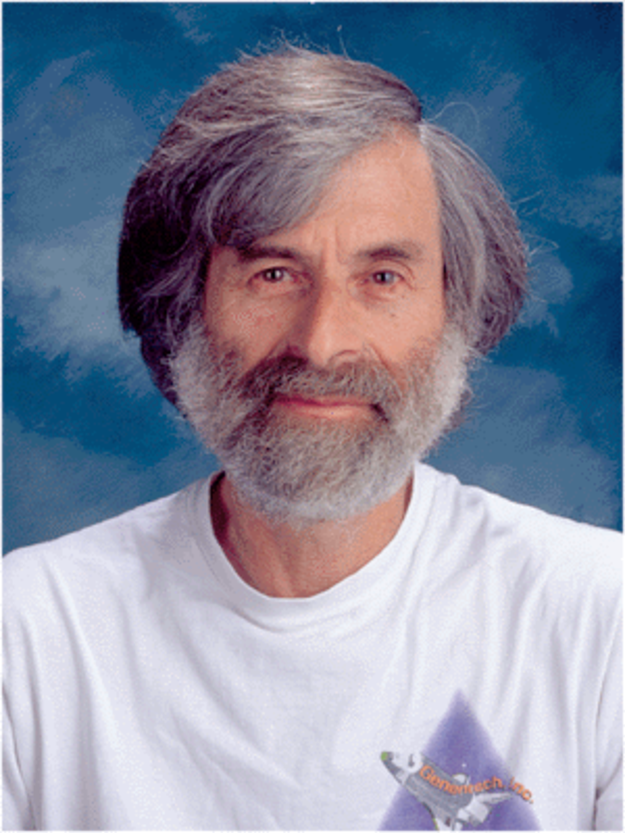
\includegraphics[width=\linewidth]{figs/leslie}
  \end{minipage}
  \hfill
  \begin{minipage}{.6\linewidth}
    \raggedright
    \begin{small}
      PhD 1972 (Brandeis University), Mathematics

      \begin{itemize}
      \item Mitre Corporation, 1962--65
      \item Marlboro College, 1965--69
      \item Massachusets Computer Associates, 1970--77
      \item SRI International, 1977--85
      \item Digital Equipment Corporation/Compaq, 1985--2001
      \item Microsoft Research, since 2001
      \end{itemize}
    \end{small}
  \end{minipage}

\bigskip

  Pioneer of distributed algorithms

  \begin{small}
  \begin{itemize}
  \item Natl. Academy of Engineering,
    PODC Influential Paper Award, ACM SIGOPS Hall of Fame, LICS Award,
    IEEE John v. Neumann medal, \ldots
  \item honorary doctorates (Rennes, Kiel, Lausanne, Lugano, Nancy)
  \end{itemize}
  \end{small}
\end{frame}

\begin{frame}
  \frametitle{\tlaplus{} specification language\hspace*{1.5cm}{\normalsize\url{http://tlaplus.net}}}

  \begin{minipage}{0.27\linewidth}
    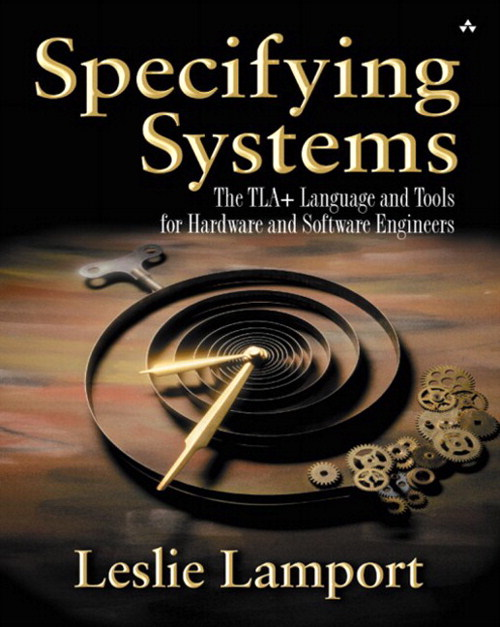
\includegraphics[width=\linewidth]{figs/tla-book-cover}
  \end{minipage}
  \hfill
  \begin{minipage}{.7\linewidth}
    \raggedright

    \begin{small}
    \begin{itemize}
    \item formal language for describing and reasoning about
      distributed and concurrent systems
\medskip
    \item based on mathematical logic and set theory\\
      plus linear time temporal logic TLA
\medskip
    \item book: Addison-Wesley, 2003\\
      (free download for personal use)
\medskip
    \item supported by tool set (\tlaplus{} toolbox)      
    \end{itemize}
    \end{small}
  \end{minipage}

  \pause
  \bigskip

  \tc{dkblue}{Some other publications}

  \begin{footnotesize}
  \begin{itemize}
  \item Y. Yu, P. Manolios, L. Lamport: \emph{Model checking \tlaplus{}
      Specifications}. CHARME 1999, pp. 54-66, LNCS 1703.
  \item S. Merz: \emph{The Specification Language \tlaplus}. In: Logics of
    Specification Languages (D. Bj{\slasho}rner, M. Henson, eds.), Springer
    2008, pp. 401-451.
  \item K. Chaudhuri, D. Doligez, L. Lamport, S. Merz: \emph{Verifying Safety
    Properties with the \tlaplus{} Proof System}. IJCAR 2010, pp. 142-148, LNCS 6173
  \end{itemize}
  \end{footnotesize}
\end{frame}

\begin{frame}
  \frametitle{A Sequential Algorithm}

  \begin{itemize}
  \item \tc{dkblue}{Pseudo-code of Euclid's algorithm}

    \bigskip

    \hspace*{4em}
    \begin{minipage}{.5\linewidth}\small
    \begin{tabbing}
      \quad\=\quad\=\textbf{then }\=\kill
      \textbf{variables} $x = M, y = N$\\
      \textbf{begin}\\
      \> \textbf{while} $x \neq y$ \textbf{do}\\
      \>\> \textbf{if} $x<y$\\
      \>\> \textbf{then}\> $y := y-x$\\
      \>\> \textbf{else}\> $x := x-y$\\
      \>\> \textbf{end if}\\
      \> \textbf{end while};\\
      \> \textbf{assert} $x = GCD(M,N)$\\
      \textbf{end}
    \end{tabbing}
    \end{minipage}

  \oo \tc{dkblue}{This is a legal PlusCal algorithm}

    \begin{itemize}
    \o embedded in a \tlaplus\ module defining $GCD$
    \o can be model checked, for fixed values of $M$ and $N$
    \end{itemize}
  \end{itemize}
\end{frame}

\begin{frame}
  \frametitle{Euclid's Algorithm in \tlaplus\ (1/2)}

  \begin{itemize}
  \item \tc{dkblue}{We start by defining divisibility and $GCD$}

    \medskip

    \begin{tlablock}
      \begin{minipage}{.96\linewidth}
      \begin{nomodule}
        \topbar{Euclid}
        \EXTENDS\ Naturals\\[1mm]
        \(\begin{noj}
          PosInteger\ \deq\ Nat \setminus \{0\}\\
          Maximum(S)\ \deq\ \CHOOSE\ x \in S : \A y \in S : x \geq y\\
          d\, |\, q\ \deq\ \E k \in 1\,..\,q : q = k * d
          \quad\quad\quad\comment{definition of divisibility}\\
          Divisors(q)\ \deq\ \{d \in 1\,..\,q : d\, |\, q\}
          \quad\ \,\comment{set of divisors}\\
          GCD(p,q)\ \deq\ Maximum(Divisors(p) \cap Divisors(q))
        \end{noj}\)\\
        \midbar
      \end{nomodule}
      \end{minipage}
    \end{tlablock}

  \oo \tc{dkblue}{Standard mathematical definitions}

    \begin{itemize}
    \o \tlaplus\ is based on (untyped) set theory
    \o simple module language for structuring larger specification
    \o import \tlaplus\ library module $Naturals$ for basic arithmetic
    \o \tlaplus\ module contains declarations, assertions, and definitions
    \end{itemize}

%  \oo \tc{dkblue}{These definitions could go to a library module}
  \end{itemize}
\end{frame}

\begin{frame}
  \frametitle{Euclid's Algorithm in \tlaplus\ (2/2)}

  \begin{itemize}
  \item \tc{dkblue}{Now model the algorithm and assert its correctness}

    \medskip

    \begin{tlablock}
      \begin{minipage}{.96\linewidth}
      \begin{nomodule}
        \CONSTANTS\ \ M, N\\
        \ASSUME\ \ $Positive\ \deq\ M \in PosInteger \land N \in PosInteger$
        \hspace{3mm}\only<2>{\makebox[0cm][l]{\raisebox{1mm}[0pt][0pt]{\begin{minipage}{2.4cm}
          \begin{beamercolorbox}[rounded=true,shadow=true]{postit}\footnotesize
            \textsf{\alert{constant formula}}
          \end{beamercolorbox}
        \end{minipage}}}}\\
        \VARIABLES\ \ x, y\\[1mm]
        \(\begin{array}{@{}l@{\ \ }c@{\ \ }l}
          Init & \deq & x=M \land y=N
        \hspace{4mm}\only<2>{\makebox[0cm][l]{\raisebox{2mm}[0pt][0pt]{\begin{minipage}{1.9cm}
          \begin{beamercolorbox}[rounded=true,shadow=true]{postit}\footnotesize
            \textsf{\alert{state formula}}
          \end{beamercolorbox}
        \end{minipage}}}}\\
          SubX & \deq & x<y \land y' = y-x \land x' = x
        \hspace{4mm}\only<2>{\makebox[0cm][l]{\raisebox{-2mm}[0pt][0pt]{\begin{minipage}{2.2cm}
          \begin{beamercolorbox}[rounded=true,shadow=true]{postit}\footnotesize
            \textsf{\alert{action formulas}}
          \end{beamercolorbox}
        \end{minipage}}}}\\
          SubY & \deq & y<x \land x' = x-y \land y' = y\\
          Spec & \deq & Init \land \alw[SubX \lor SubY]_{\seq{x,y}}
        \hspace{5mm}\only<2>{\makebox[0cm][l]{\raisebox{0mm}[0pt][0pt]{\begin{minipage}{2.4cm}
          \begin{beamercolorbox}[rounded=true,shadow=true]{postit}\footnotesize
            \textsf{\alert{temporal formula}}
          \end{beamercolorbox}
        \end{minipage}}}}\\
        \end{array}\)\\
        \midbar
        $Correctness\ \deq\ x=y \implies x = GCD(M,N)$\\[1mm]
        \THEOREM\ \ $Spec \implies \alw Correctness$\\
        \bottombar
      \end{nomodule}
      \end{minipage}
    \end{tlablock}

  \oo \tc{dkblue}{Transitions represented by action formulas $SubX$, $SubY$}

  \oo \tc{dkblue}{Algorithm represented by initial condition and next-state relation}

  \oo \tc{dkblue}{Correctness expressed as TLA formula}
  \end{itemize}
\end{frame}

% \begin{frame}
%   \frametitle{\tlaplus\ Modules}

%   \begin{itemize}
%   \item \tc{dkblue}{\tlaplus\ specifications are structured in modules}

%     \begin{itemize}
%     \o structured specifications: import existing modules via \EXTENDS
%     \o \tlaplus\ also provides \INSTANCE\ for import with renaming
%     \end{itemize}

%   \oo \tc{dkblue}{Modules contain declarations, definitions, and assertions}

%     \begin{itemize}
%     \o declarations of \CONSTANTS\ and \VARIABLES
%     \o main body of module: operator definitions
%     \o assertions of facts: \ASSUME\ and \THEOREM
%     \end{itemize}

%   \oo \tc{dkblue}{Levels of formulas and operators}

%     \medskip

%     \renewcommand{\arraystretch}{1.2}
%     \quad{\small\begin{tabular}{l@{\qquad}l@{\qquad}l}
%         \alert{constant} & only \CONSTANT\ symbols & \tc{dkgreen}{$Positive$}\\
%         \alert{state} & allow \VARIABLE{}s & \tc{dkgreen}{$Init,\ Correctness$}\\
%         \alert{action} & allow primed \VARIABLE{}s & \tc{dkgreen}{$SubX, SubY$}\\
%         \alert{temporal} & use temporal operators & \tc{dkgreen}{$Spec$}
%     \end{tabular}}
%   \end{itemize}
% \end{frame}

\begin{frame}
  \frametitle{Verification of Euclid's Algorithm: Model Checking}

  \begin{itemize}
  \item \tc{dkblue}{\tlc\ : explicit-state model checker}

    \begin{itemize}
    \o verify correctness properties for finite instances
    \o Euclid: fix concrete values for $M$ and $N$
    \o check that the result is correct for these inputs
    \end{itemize}

  \oo \tc{dkblue}{Variation: verify correctness over fixed interval}

  \oo \alert{Invaluable for debugging \tlaplus\ models}

    \begin{itemize}
    \o verify many seemingly trivial properties
    \o type correctness, executability of every individual action, \ldots
    \o absence of deadlock, eventual response to requests, \ldots
    \o reveal corner cases before attempting full correctness proof
    \end{itemize}
  \end{itemize}

\end{frame}

\section{Theorem Proving With \tlaps}

\begin{frame}
  \frametitle{Using \tlaps\ to Prove Euclid's Algorithm Correct}

  \begin{itemize}
  \item \tc{dkblue}{Verify correctness for all possible inputs}

  \oo \tc{dkblue}{\tlaps: proof assistant for verifying \tlaplus\ specifications}

    \begin{itemize}
    \o interesting specifications cannot be verified fully automatically
    \o user provides proof (skeleton) to guide verification
    \o automatic back-end provers discharge leaf obligations
    \end{itemize}

\pause

  \oo \tc{dkblue}{Application to Euclid's algorithm}

    \begin{itemize}
    \o first step: strengthen correctness property $\leadsto$ \alert{inductive invariant}

       \medskip
       \begin{tlablock}[.7]
         InductiveInvariant\ \deq\ 
         \begin{conj}
           x \in PosInteger\\
           y \in PosInteger\\
           GCD(x,y) = GCD(M,N)
         \end{conj}
       \end{tlablock}
    \end{itemize}
  \end{itemize}
\end{frame}

\begin{frame}
  \frametitle{Underlying Data Properties}

  \begin{itemize}
  \item \tc{dkblue}{The algorithm relies on the following properties of $GCD$}

     \bigskip

     \begin{tlablock}
       \begin{array}{@{}l@{\ \ }c@{\ \ }l}
         \THEOREM\ \ GCDSelf & \deq &
         \begin{array}[t]{@{}l@{\ \ }l}
           \ASSUME & \NEW\ p \in PosInteger\\
           \PROVE  & GCD(p,p) = p
         \end{array}\vspace{2mm}\\ 
         \THEOREM\ \ GCDSymm & \deq &
         \begin{array}[t]{@{}l@{\ \ }l}
           \ASSUME & \NEW\ p \in PosInteger,\\
                   & \NEW\ q \in PosInteger\\
           \PROVE  & GCD(p,q) = GCD(q,p)
         \end{array}\vspace{2mm}\\
         \THEOREM\ \ GCDDiff & \deq &
         \begin{array}[t]{@{}l@{\ \ }l}
           \ASSUME & \NEW\ p \in PosInteger,\\
                   & \NEW\ q \in PosInteger,\\
                   & p<q\\
           \PROVE  & GCD(p,q) = GCD(p, q-p)
         \end{array}
       \end{array}
     \end{tlablock}

  \oo \tc{dkblue}{$\ASSUME$ \ldots\ $\PROVE$ : \tlaplus\ notation for sequents}

  \oo \tc{dkblue}{We won't bother proving these properties here}
  \end{itemize}
\end{frame}

\begin{frame}
  \frametitle{Invariant Proofs in \tlaplus}

  \begin{itemize}
  \item \tc{dkblue}{Establish an invariant in \tlaplus}

    \medskip

\begin{center}
  \renewcommand{\arraystretch}{1.2}
    \qquad\(\color{dkgreen}\begin{array}{c}
      Init \implies Inv \quad Inv \land [Next]_v \implies Inv' \quad Inv \implies Corr\\
      \hline
      Init \land \alw[Next]_v \implies \alw Corr
    \end{array}\)
\end{center}

    \begin{itemize}
    \o $Inv$ is true initially, is preserved by all steps, and implies $Corr$
    \end{itemize}

\pause

  \o \tc{dkblue}{Formal representation as the following sequent}

     \medskip

     \qquad\begin{tlablock}
       \THEOREM\ \ ProveInv\ \deq\ 
       \begin{array}[t]{@{}l@{\ \ }l}
         \ASSUME & \STATE\ Init,\ \STATE\ Inv,\ \STATE\ Corr,\\
                 & \ACTION\ Next,\ \STATE\ v,\\
                 & Init \implies Inv,\\
                 & Inv \land [Next]_v \implies Inv',\\
                 & Inv \implies Corr\\
         \PROVE  & Init \land \alw[Next]_v \implies \alw Corr
       \end{array}
     \end{tlablock}

     \begin{itemize}
     \o \tlaps\ doesn't handle temporal logic yet \ldots
     \o \ldots\ but it can be used to establish the non-temporal hypotheses
     \end{itemize}
  \end{itemize}
\end{frame}

\begin{frame}
  \frametitle{Simple Proofs}

  \begin{itemize}
  \item \tc{dkblue}{Prove that $InductiveInvariant$ implies $Correctness$}

    \medskip

    \qquad\begin{tlablock}
      \LEMMA\ \ InductiveInvariant \implies Correctness\\
      \only<1>{\alert{\OBVIOUS}}
      \only<2->{\BY\ GCDSelf\ \DEFS\ InductiveInvariant, Correctness}
    \end{tlablock}

\pause



    \begin{itemize}
    \o \tlaps\ requires definitions and facts to be cited explicitly
    \o this helps manage the size of the search space for backend provers
    \end{itemize}

\pause
  \oo \tc{dkblue}{Prove that $Init$ implies $InductiveInvariant$}

    \medskip

    \qquad\begin{tlablock}
      \LEMMA\ \ Init \implies InductiveInvariant\\
      \BY\ Positive\ \DEFS\ Init, InductiveInvariant
    \end{tlablock}

  \oo \tc{dkblue}{Proving simple theorems: expand definitions, cite lemmas}
  \end{itemize}
  
\end{frame}

\begin{frame}
  \frametitle{Hierarchical Proofs}

  \begin{itemize}
  \item \tc{dkblue}{Complex proofs consist of a sequence of claims, ending with \QED}

  \oo \tc{dkblue}{Prove that all transitions preserve $InductiveInvariant$}

    \medskip

    \qquad\begin{tlablock}[.88]
      \LEMMA\ \ InductiveInvariant \land [SubX \lor SubY]_{\seq{x,y}} \implies InductiveInvariant'\\
\onslide<2->{
      \ps{1}{}\ \USE\ \DEF\ InductiveInvariant
  }\\
\onslide<3->{
      \ps{1}{1.}\ 
        \begin{array}[t]{@{}l@{\ \ }l}
          \ASSUME & InductiveInvariant, SubX\\
          \PROVE  & InductiveInvariant'
        \end{array}\\
      \ps{1}{2.}\ 
        \begin{array}[t]{@{}l@{\ \ }l}
          \ASSUME & InductiveInvariant, SubY\\
          \PROVE  & InductiveInvariant'
        \end{array}
  }\\
\onslide<4->{
      \ps{1}{q.}\ \QED\\
      \quad  \quad \BY\ \ps{1}{1}, \ps{1}{2}
  }
    \end{tlablock}

\onslide<2->{
    \begin{itemize}
    \o \only<2>{\USE\ \DEF\ causes \tlaps\ to silently expand definitions}
       \only<3>{The steps $\ps{1}{1}$ and $\ps{1}{2}$ will be proved subsequently}
       \only<4>{\QED\ step verifies that the lemma follows from above steps ---\\
                includes trivial case $\UNCHANGED \seq{x,y}$}
    \end{itemize}
  }
  \end{itemize}
\end{frame}



\begin{frame}
  \frametitle{Hierarchical Proofs: Sublevels}

    \qquad\begin{tlablock}
      {\color{gray}(...)} \\
      \ps{1}{1.}\ 
        \begin{array}[t]{@{}l@{\ \ }l}
          \ASSUME & InductiveInvariant, SubX\\
          \PROVE  & InductiveInvariant'
        \end{array}\\
\onslide<2->{
      \quad \ps{2}{1.}\ x' \in PosInteger \land y' \in PosInteger
}\\
\onslide<3->{
      \quad\quad \BY\ \ps{1}{1},\ SimpleArithmetic\ \DEF\ PosInteger, SubX
}\\
\onslide<2->{
  	\quad \ps{2}{2.}\  \QED\\
        \quad\quad \BY\ \ps{1}{1}, \ps{2}{1},\ GCDDiff\ \DEF\ SubX
}\\
      \ps{1}{2.}\ 
        \begin{array}[t]{@{}l@{\ \ }l}
          \ASSUME & InductiveInvariant, SubY\\
          \PROVE  & InductiveInvariant'
        \end{array}\\
 {\color{gray}(...)} 
    \end{tlablock}
    
\uncover<3->{
  \begin{itemize}
  \oo \tc{dkblue}{Cited fact $SimpleArithmetic$}

    \begin{itemize}
    \o theorem from the standard module TLAPS
    \o invokes decision procedure for Presburger arithmetic 
    \end{itemize}
  \end{itemize}
}

\end{frame}


\section{The \tlaplus\ Proof Language}

\begin{frame}
  \frametitle{Assertions (in Modules or Proofs)}

  \begin{itemize}
  \item \tc{dkblue}{Assertions state validity of formulas in current context}

  \oo \tc{dkblue}{\AXIOM\ and \ASSUME\ assert unproved facts}

    \begin{itemize}
    \o \tlaps\ handles \ASSUME\ and \AXIOM\ identically
    \o \tlc\ checks \ASSUME{}d facts
    \end{itemize}

  \oo \tc{dkblue}{\THEOREM\ asserts that a fact is provable in the current context}

    \begin{itemize}
    \o proofs can be filled in later
    \o GUI reflects proof status (missing, incomplete, finished)
%    \o \LEMMA\ and \PROPOSITION\ are synonyms of \THEOREM
    \end{itemize}

  \oo \tc{dkblue}{Facts can be named for future reference}

    \medskip

    \begin{tlablock}[.89]
      \THEOREM\ Fermat\ \deq\ \forall n \in Nat \setminus (0..2): \forall a,b,c \in Nat \setminus \{0\}: a^n + b^n \neq c^n
    \end{tlablock}

  \end{itemize}
\end{frame}

\begin{frame}
  \frametitle{Shape of Non-Temporal Assertions}

  \begin{itemize}
  \item \tc{dkblue}{A \tlaplus\ assertion can be a formula or a logical sequent}

    \medskip

    \qquad\begin{tlablock}[.7]
      \qquad $F$
      \qquad\qquad\text{or}\qquad\qquad
      \begin{array}{@{}l@{\ \ }l}
        \ASSUME & A_1, \ldots, A_n\\
        \PROVE  & F
      \end{array}
    \end{tlablock}

  \oo \tc{dkblue}{Shape of a sequent \ASSUME\ \ldots\ \PROVE}

    \begin{itemize}
    \o the conclusion $F$ is always a formula

    \o the assumptions $A_i$ can be 

      \medskip

      \begin{tabular}{@{}ll}
        declarations & \tc{dkgreen}{$\NEW\ msg \in Msgs$}\\
                     & (levels: \CONSTANT, \STATE, \ACTION, \TEMPORAL)\\[2mm]
        formulas & \tc{dkgreen}{$msg.type = \str{alert}$}\\[2mm]
        sequents & 
        \tc{dkgreen}{\(\begin{array}[t]{@{}l@{\ \ }l}
          \ASSUME & \NEW\ msg \in Msgs,\ msg.type = \str{alert}\\
          \PROVE  & msg \in Alarm
        \end{array}\)}
      \end{tabular}
    \end{itemize}
  \end{itemize}
\end{frame}

\begin{frame}
  \frametitle{Nested \ASSUME\ \ldots\ \PROVE\ Sequents}

  \begin{itemize}
  \item \tc{dkblue}{Nested sequents are useful for writing proof rules}

    \bigskip

    \begin{tlablock}
      \THEOREM\ ForallIntro\ \deq
      \begin{array}[t]{l@{\ \ }l}
        \ASSUME & \NEW\ P(\_),\\
                & \ASSUME\ \ \NEW\ y\ \ \PROVE\ \ P(y)\\
        \PROVE  & \A x : P(x)
      \end{array}
    \end{tlablock}

    \bigskip

    \begin{itemize}
    \item nested \ASSUME\ \ldots\ \PROVE\ encodes freshness of $y$
    \end{itemize}

  \end{itemize}
\end{frame}

\begin{frame}
  \frametitle{The Proof Language}

  \begin{itemize}
  \item \tc{dkblue}{Hierarchically nested sequents}

    \begin{itemize}
    \o standard forward-style reasoning
    \o final \QED\ step proves enclosing assertion, using preceding steps
    \end{itemize}

  \oo \tc{dkblue}{\SUFFICES\ steps for backward reasoning}

    \begin{itemize}
    \o \tc{dkgreen}{$\SUFFICES\ \varphi$} : show that $\varphi$ implies current goal
    \o make $\varphi$ current goal for the remainder of current scope
    \end{itemize}

  \oo \tc{dkblue}{Using and hiding definitions and facts}

    \begin{itemize}
    \o in $\BY$ proof or for remainder of current scope
    \end{itemize}

  \oo \tc{dkblue}{A few derived forms for convenience}

    \begin{itemize}
    \o reasoning patterns for basic connectives: $\implies$, $\forall$, $\exists$
    \end{itemize}
  \end{itemize}
\end{frame}

% \begin{frame}
%   \frametitle{\tlaps\ vs. Other Proof Assistants}

%   \begin{itemize}
%   \item \tc{dkblue}{\tlaps\ does not hard-wire a full proof calculus}

%     \begin{itemize}
%     \o library module TLAPS.tla contains \tlaplus\ proof rules
%     \end{itemize}

%   \oo \tc{dkblue}{User is free to give structure of correctness argument}

%     \begin{itemize}
%     \o provability of leaf assertions defined by back-end provers
%     \o use of different back-ends (ideally) transparent to user
%     \o \QED\ step verifies provability of overall assertion
%     \end{itemize}

%   \oo \tc{dkblue}{Declarative, hierarchical proofs}

%     \begin{itemize}
%     \o current context defines set of known facts and definitions
%     \o explicit statement of current assertion, unlike tactic proofs
%     \o explicit citations of used facts and definitions
%     \o improve readability and ensure manageability of proof state
%     \end{itemize}
%   \end{itemize}
% \end{frame}

\begin{frame}
  \frametitle{Architecture of \tlaps}

  \centerline{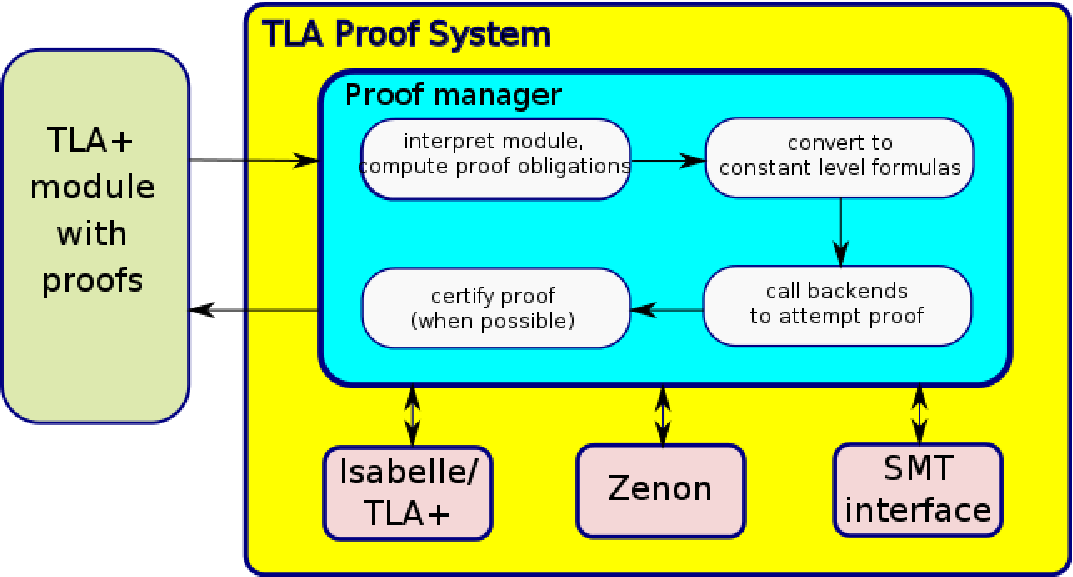
\includegraphics[width=1.0\linewidth]{figs/architecture}}
\end{frame}

\begin{frame}
  \frametitle{Proof Manager}

  \begin{itemize}
  \item \tc{dkblue}{Interprets \tlaplus\ proof language, computes proof obligations}

    \begin{itemize}
    \o track module structure (imports and instantiations)
    \o manage context: known and usable facts and definitions
    \o expand operator definitions if they are usable
    \end{itemize}

  \oo \tc{dkblue}{Rewrites proof obligations to constant level}

    \begin{itemize}
    \o handle primed expressions such as\ \ \tc{dkgreen}{$Inv'$}
    \o distribute prime over (constant-level) operators
    \o introduce distinct symbols \tc{dkgreen}{$e$} and \tc{dkgreen}{$e'$}
       for atomic state expression \tc{dkgreen}{$e$}
    \end{itemize}

  \oo \tc{dkblue}{Invokes backend provers}

    \begin{itemize}
    \o user may explicitly indicate which proof method to apply
    \o optionally: certify backend proof using Isabelle/\tlaplus
    \end{itemize}
  \end{itemize}
\end{frame}

\begin{frame}
  \frametitle{Temporal Proofs (1)}

  \begin{itemize}
  \item \tc{dkblue}{The problem with temporal (modal) reasoning}

    \begin{itemize}
    \o temporal formulas are interpreted over current (implicit) behavior
    \o \makebox[1.65cm][l]{\tc{dkgreen}{$F \vdash G$}} 
       deduce validity of $G$ from validity of $F$
       \hfill
       \uncover<2->{\raisebox{-1mm}{\makebox[2cm][l]{\tlabox{1.6cm}{$F \vdash \Box F$}}}}
    \o \makebox[1.65cm][l]{\tc{dkgreen}{$\vdash F \implies G$}}
       implication holds in current behavior
       \unitlength 1mm
       \hfill
       \uncover<2->{\raisebox{-1mm}{%
         \makebox[0cm][l]{\tlabox{1.6cm}{$\vdash F \implies \Box F$}}%
         \alert{\begin{picture}(20,4)\put(-2,5){\line(4,-1){20}}\put(-2,0){\line(4,1){20}}\end{picture}}%
       }}

    \medskip

    \o standard calculi rely on identification of these sequents
    \end{itemize}

\onslide<3->

  \oo \tc{dkblue}{Possible solution: introduce explicit parameters}

    \begin{itemize}
    \o distinguish\ \ \tc{dkgreen}{$\sigma \models F \implies G$}\ \ and\ \ 
       \tc{dkgreen}{$(\forall \sigma: \sigma \models F) \vdash (\forall \tau: \tau \models G)$}
    \o also need relation\ \ \tc{dkgreen}{$\sigma \sqsubseteq \tau$}
       for ``transferring'' temporal formulas
    \end{itemize}

  \oo \alert{Sound, but contrary to the spirit of temporal logic}
  \end{itemize}
\end{frame}

\begin{frame}
  \frametitle{Temporal Proofs (2)}

  \begin{itemize}
  \item \tc{dkblue}{Key observations}

    \begin{itemize}
    \o implicit behavior at lower levels is a suffix of that at higher levels
    \o an assumption $\Box F$ is usable throughout the entire subproof
    \o \tc{dkgreen}{$\Box F \vdash G$}\ \ coincides with\ \ 
       \tc{dkgreen}{$\vdash \Box F \implies G$}
    \end{itemize}

  \oo \tc{dkblue}{Distinguish temporal sequents in \tlaplus\ proofs}

    \medskip

    {\small
    \qquad\(\color{dkgreen}
    \begin{array}[t]{@{}l@{\ \ }l@{\qquad\qquad}l}
      \TASSUME & F  & \text{\tc{black}{assume that $F$ is true for all suffixes \ldots}}\\[1mm]
      \TPROVE  & G  & \text{\tc{black}{\ldots\ then prove $G$ for a fresh suffix}}
    \end{array}
    \)
    }

  \oo \tc{dkblue}{Proof structure}

    \begin{itemize}
    \o upper levels state temporal sequents, lower levels ordinary ones
    \o temporal sequents never occur in the scope of ordinary ones
    \o all assumptions remain usable throughout the subproof
    \end{itemize}
  \end{itemize}
\end{frame}

\begin{frame}
  \frametitle{Temporal Proof Rules}

  \centerline{\begin{tlablock}[.6]
      \THEOREM\ Inv1\ \deq\ 
      \begin{array}[t]{@{}l@{\ \ }l}
        \TASSUME & \STATE\ Inv,\\
                 & Inv \implies Inv'\\
        \TPROVE  & Inv \implies \Box Inv
      \end{array}
  \end{tlablock}}

  \begin{itemize}
  \oo \tc{dkblue}{Use of this rule}

    \begin{itemize}
    \o next-state relation \tc{dkgreen}{$\Box[N]_v$} present among hypotheses
    \o \tc{dkgreen}{$Inv \implies Inv'$}\ \ proved as shown before, using\ \ \tc{dkgreen}{$[N]_v$}
    \o also prove\ \ \tc{dkgreen}{$Init \implies Inv$}\ \ in order to derive\ \ \tc{dkgreen}{$Spec \implies \Box Inv$}
    \end{itemize}

\pause

  \oo \tc{dkblue}{Substantial simplification of temporal verification rules}

    \medskip
    \centerline{\begin{tlablock}[.85]
        \THEOREM\ SF1\ \deq\ 
        \begin{array}[t]{@{}l@{\ \ }l}
          \TASSUME & \STATE\ P,\ \STATE\ Q,\ \STATE\ f,\ \ACTION\ A,\\
                   & \SF_f(A),\\
                   & P \implies P' \lor Q',\\
                   & P \land \an{A}{f} \implies Q',\\
                   & \Box P \implies \eve \ENABLED\,\an{A}{f}\\
          \TPROVE  & P \leadsto Q
        \end{array}
    \end{tlablock}}
  \end{itemize}
\end{frame}

\section{Conclusions}

\begin{frame}
  \frametitle{Present and \alert{future} of the \tlaps}

  \begin{itemize}
  \item \tc{dkblue}{Current release: october 2010}

    \begin{itemize}
%    \o \url{http://msr-inria.inria.fr/~doligez/tlaps/}
    \o releases (source and binary) include back-end provers
    \o Eclipse-based GUI (\tlaplus\ toolbox) for non-linear interaction
    \end{itemize}

  \oo \tc{dkblue}{Restricted to proving non-temporal properties}

    \begin{itemize}
    \o invariant and step simulation (refinement) proofs
    \o carried out several case studies, some contained in distribution
    \end{itemize}

  \oo \alert{Support for temporal logic (liveness properties)}

    \begin{itemize}
    \o implement support for temporal sequents in proof manager
    \o encode semantics of temporal logic in Isabelle/\tlaplus
    \end{itemize}

  \oo \alert{More backend provers}

    \begin{itemize}
    \o SMT solver, eventually with proof reconstruction
    \o better support for standard theories (arithmetic, sequences, \ldots)
    \end{itemize}

  \oo \alert{Looking forward to user feedback}
  \end{itemize}
\end{frame}

\end{document}

%%% Local Variables: 
%%% mode: latex
%%% TeX-master: t
%%% End: 
